% Options for packages loaded elsewhere
\PassOptionsToPackage{unicode}{hyperref}
\PassOptionsToPackage{hyphens}{url}
%
\documentclass[
]{article}
\usepackage{amsmath,amssymb}
\usepackage{lmodern}
\usepackage{iftex}
\ifPDFTeX
  \usepackage[T1]{fontenc}
  \usepackage[utf8]{inputenc}
  \usepackage{textcomp} % provide euro and other symbols
\else % if luatex or xetex
  \usepackage{unicode-math}
  \defaultfontfeatures{Scale=MatchLowercase}
  \defaultfontfeatures[\rmfamily]{Ligatures=TeX,Scale=1}
\fi
% Use upquote if available, for straight quotes in verbatim environments
\IfFileExists{upquote.sty}{\usepackage{upquote}}{}
\IfFileExists{microtype.sty}{% use microtype if available
  \usepackage[]{microtype}
  \UseMicrotypeSet[protrusion]{basicmath} % disable protrusion for tt fonts
}{}
\makeatletter
\@ifundefined{KOMAClassName}{% if non-KOMA class
  \IfFileExists{parskip.sty}{%
    \usepackage{parskip}
  }{% else
    \setlength{\parindent}{0pt}
    \setlength{\parskip}{6pt plus 2pt minus 1pt}}
}{% if KOMA class
  \KOMAoptions{parskip=half}}
\makeatother
\usepackage{xcolor}
\usepackage[margin=1in]{geometry}
\usepackage{graphicx}
\makeatletter
\def\maxwidth{\ifdim\Gin@nat@width>\linewidth\linewidth\else\Gin@nat@width\fi}
\def\maxheight{\ifdim\Gin@nat@height>\textheight\textheight\else\Gin@nat@height\fi}
\makeatother
% Scale images if necessary, so that they will not overflow the page
% margins by default, and it is still possible to overwrite the defaults
% using explicit options in \includegraphics[width, height, ...]{}
\setkeys{Gin}{width=\maxwidth,height=\maxheight,keepaspectratio}
% Set default figure placement to htbp
\makeatletter
\def\fps@figure{htbp}
\makeatother
\setlength{\emergencystretch}{3em} % prevent overfull lines
\providecommand{\tightlist}{%
  \setlength{\itemsep}{0pt}\setlength{\parskip}{0pt}}
\setcounter{secnumdepth}{-\maxdimen} % remove section numbering
\usepackage{fontspec}
\setmainfont{Timenewroman}
\usepackage{setspace}
\setstretch{1.5}
\ifLuaTeX
  \usepackage{selnolig}  % disable illegal ligatures
\fi
\IfFileExists{bookmark.sty}{\usepackage{bookmark}}{\usepackage{hyperref}}
\IfFileExists{xurl.sty}{\usepackage{xurl}}{} % add URL line breaks if available
\urlstyle{same} % disable monospaced font for URLs
\hypersetup{
  pdfauthor={Anastasia Möller, Johannes Schadt, Sylviane Verschaeve, Tine Limberg},
  hidelinks,
  pdfcreator={LaTeX via pandoc}}

\title{\Huge~\textbf{Final Report:} Proteome-wide Screen for
RNA-dependent Proteins\\
\emph{non-synchronized A549 cells}}
\author{Anastasia Möller, Johannes Schadt, Sylviane Verschaeve, Tine
Limberg}
\date{17.07.2023}

\begin{document}
\maketitle

{
\setcounter{tocdepth}{2}
\tableofcontents
}
Loading the data:

\hypertarget{introduction}{%
\section{1. Introduction}\label{introduction}}

\hypertarget{importance-of-rna-binding-proteins}{%
\subsection{1.1. Importance of RNA-binding
proteins}\label{importance-of-rna-binding-proteins}}

\hypertarget{experimental-setup}{%
\subsection{1.2. Experimental Setup}\label{experimental-setup}}

\hypertarget{methods}{%
\section{2. Methods}\label{methods}}

\hypertarget{data-cleanup}{%
\subsection{2.1. Data cleanup}\label{data-cleanup}}

\hypertarget{normalization-methods}{%
\subsection{2.2. Normalization methods}\label{normalization-methods}}

\hypertarget{reproducibility-and-batch-effect}{%
\subsection{2.3. Reproducibility and Batch
Effect}\label{reproducibility-and-batch-effect}}

\hypertarget{scaling-and-reduction-of-dataset}{%
\subsection{2.4. Scaling and Reduction of
Dataset}\label{scaling-and-reduction-of-dataset}}

\hypertarget{our-limitations-with-gaussian-fit}{%
\subsection{2.5. Our limitations with Gaussian
fit}\label{our-limitations-with-gaussian-fit}}

description of problem with local peaks and inaccuracy of overlap

Alternatively, we \ldots{}

\hypertarget{data-description-via-parameters}{%
\subsection{2.6. Data description via
Parameters}\label{data-description-via-parameters}}

The control sample and the RNase sample for each protein will be
compared via the

Via the parameters the differences between the RNase and the Control are
depicted manually via the parameters.

\hypertarget{parameter-1-significant-change-of-protein-amount-under-global-peak}{%
\subsubsection{2.6.1. Parameter 1: Significant change of protein amount
under global
peak}\label{parameter-1-significant-change-of-protein-amount-under-global-peak}}

\hypertarget{parameter-2-significant-change-of-protein-amount-under-local-peaks}{%
\subsubsection{2.6.2. Parameter 2: Significant change of protein amount
under local
peaks}\label{parameter-2-significant-change-of-protein-amount-under-local-peaks}}

\hypertarget{parameter-3-significant-fraction-shift-of-global-peak}{%
\subsubsection{2.6.3. Parameter 3: Significant fraction-shift of global
peak}\label{parameter-3-significant-fraction-shift-of-global-peak}}

\hypertarget{parameter-4-significant-difference-in-position-of-shoulderregions}{%
\subsubsection{2.6.4. Parameter 4: Significant difference in position of
shoulderregions}\label{parameter-4-significant-difference-in-position-of-shoulderregions}}

\hypertarget{precipitated-proteins}{%
\subsubsection{2.6.5. Precipitated
proteins}\label{precipitated-proteins}}

\hypertarget{k-means-clustering}{%
\subsection{2.7. K-means clustering}\label{k-means-clustering}}

\hypertarget{regression-analysis}{%
\subsection{2.8. Regression analysis}\label{regression-analysis}}

\hypertarget{results}{%
\section{3. Results}\label{results}}

\hypertarget{cleaned-dataset}{%
\subsection{3.1. Cleaned Dataset}\label{cleaned-dataset}}

\hypertarget{rna-dependent-proteins}{%
\subsection{3.2. RNA-dependent Proteins}\label{rna-dependent-proteins}}

\hypertarget{comparison-of-the-normalization-methods}{%
\subsection{3.3. Comparison of the normalization
methods}\label{comparison-of-the-normalization-methods}}

\hypertarget{k-means-clustering-1}{%
\subsection{3.3. K-means clustering}\label{k-means-clustering-1}}

\hypertarget{regression-analysis-1}{%
\subsection{3.4. Regression analysis}\label{regression-analysis-1}}

\hypertarget{comparison-with-database}{%
\subsection{3.5. Comparison with
Database}\label{comparison-with-database}}

\hypertarget{discussion}{%
\section{4. Discussion}\label{discussion}}

\hypertarget{literature}{%
\section{5. Literature}\label{literature}}

\hypertarget{check-for-missing-values}{%
\subsubsection{1.1. Check for missing
values}\label{check-for-missing-values}}

\hypertarget{check-data-format}{%
\subsubsection{1.2. Check data format}\label{check-data-format}}

\hypertarget{deleting-rows-with-only-zeros}{%
\subsubsection{1.3. Deleting rows with only
zeros}\label{deleting-rows-with-only-zeros}}

-\textgreater{} da die Summe der Zeileneinträge keines Proteins 0
entspricht, wurde ein Dataframe aus False erstellt. Einträge
ausschließlich False, werden durch die sum Funktion als 0 aufaddiert.

\hypertarget{rearranging-of-data}{%
\subsubsection{1.4. Rearranging of Data}\label{rearranging-of-data}}

\hypertarget{reordering-columns}{%
\paragraph{1.4.1. Reordering columns}\label{reordering-columns}}

\hypertarget{separate-ctrl-and-rnase}{%
\paragraph{1.4.2. Separate Ctrl and
RNase}\label{separate-ctrl-and-rnase}}

\hypertarget{reproducibility}{%
\subsection{2. Reproducibility}\label{reproducibility}}

Here we test whether the replicates are similar to each other. This
would mean, that the experiment is reproducible, thus the data is
reliable. Proteins that do not satisfy this condition will be removed
from the dataset and will not be analysed.

\hypertarget{pearson-correlation}{%
\paragraph{2.1 Pearson Correlation}\label{pearson-correlation}}

To facilitate the calculation of the correlation between each replicate,
we design 6 separate data frames, one for each replicate

Here we calculate the correlation between the replicates and put them
together in one data frame (ctrl.cor and rnase.cor) (?)

Now we eliminate proteins which have NA-correlations (this happens when
they contain replicates with only 0s). We then create new separate data
frames for each replicate.

Now we calculate the correlation of the replicates. This time the
proteins that containes replicates with only 0 are eliminated, so there
should be no NAs anymore.

The following plot shows us the general distribution of correlation.

In total we look at 3*(3680-83) correlations This has to be taken into
account, when looking at the graphs. It is import to figure out if the 3
cor are for one protein or for 3 different ones.

\begin{verbatim}
## Warning: Paket 'ggplot2' wurde unter R Version 4.2.3 erstellt
\end{verbatim}

\begin{verbatim}
## `stat_bin()` using `bins = 30`. Pick better value with `binwidth`.
\end{verbatim}

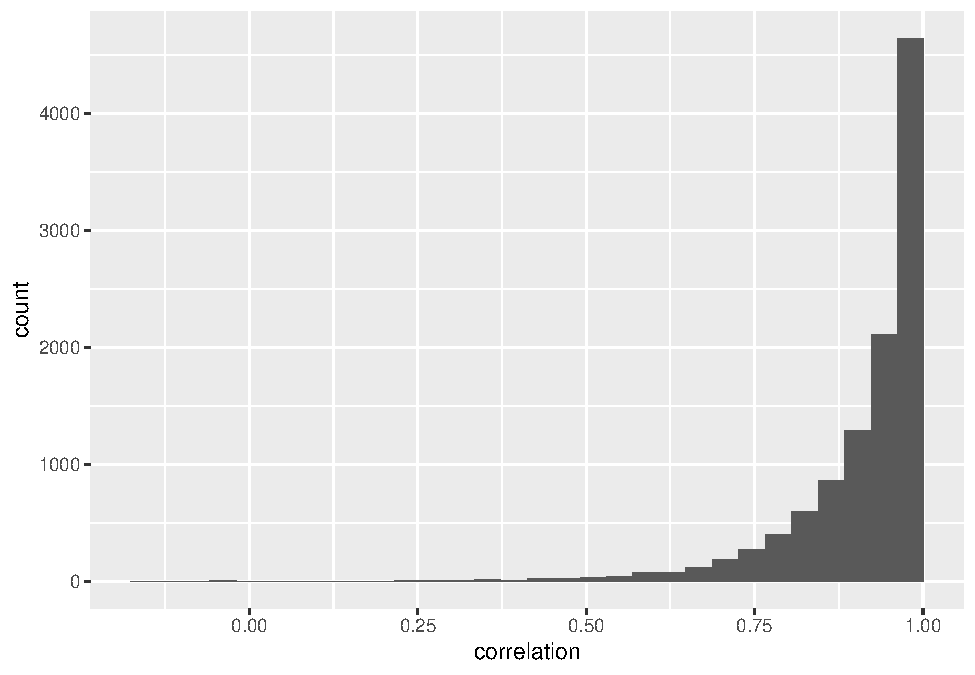
\includegraphics{Latextry_files/figure-latex/unnamed-chunk-11-1.pdf}

We do the same for the RNase group:

\begin{verbatim}
## `stat_bin()` using `bins = 30`. Pick better value with `binwidth`.
\end{verbatim}

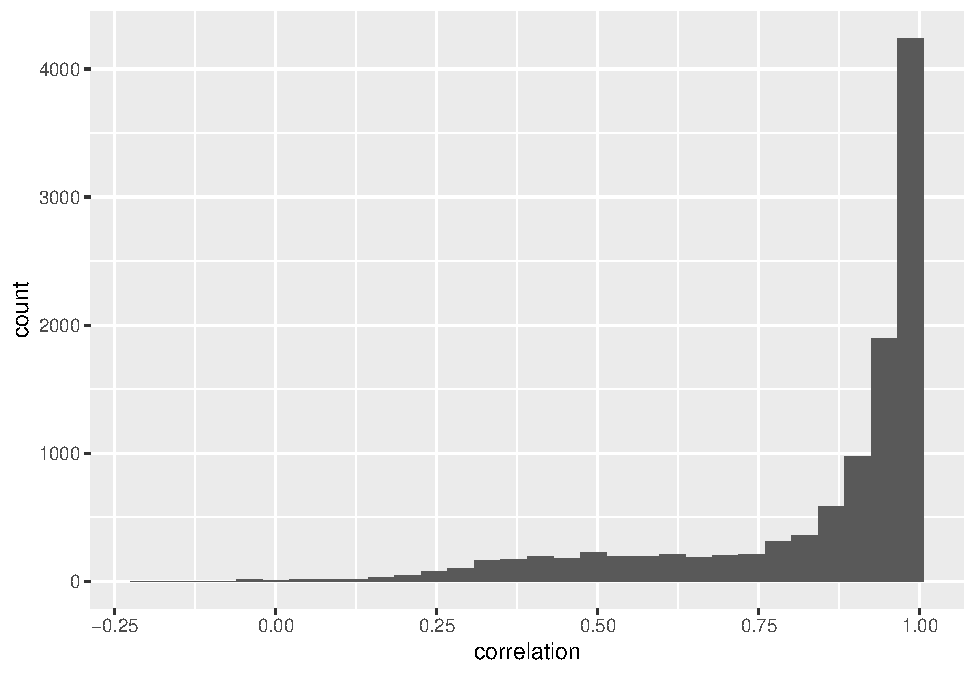
\includegraphics{Latextry_files/figure-latex/unnamed-chunk-12-1.pdf}

Now we select the proteins which have correlations beneath 0.9. Those
are not reproducible, thus the data is not safe enough to be used
further.

First we determine the proteins that only have correlations under 0.9.

Now we eliminate the proteins that only have correlations under 0.9.

Other proteins are a bit trickier. Some proteins have two replicates
similar to each other (correlation \textless{} 0.9) and a third one that
completely differs. These Proteins have one very high and two smaller
correlations. The different replicate is often the third one (mabye
batch effect). To avoid loosing too many proteins and still to still
have safe data, we try to ignore the bad replicates. For this we first
set them to NA: After the normalization-set we can ignore them.

We now have 3074 Proteins left. They are stored in new variables:

We now have clean data, with proteins that have reproducible data we can
use for further analysis.

\hypertarget{scaled-and-reduced-dataset}{%
\subsection{3. Scaled and Reduced
Dataset}\label{scaled-and-reduced-dataset}}

For the normalization each replicate has to be separated, therefore we
design 6 separate dataframes.

\hypertarget{mean-value-method}{%
\subsubsection{3.1. Mean Value Method}\label{mean-value-method}}

\hypertarget{normalization}{%
\paragraph{3.1.1. Normalization}\label{normalization}}

We perform the mean-value-method (mvm) on each replicate, both control
and RNase:

\hypertarget{reduction}{%
\paragraph{3.1.2. Reduction}\label{reduction}}

To reduce we take the mean value between each replicate. Here we must
consider the NA-values of non-reproducible replicates.

\hypertarget{scaling}{%
\paragraph{3.1.3. Scaling}\label{scaling}}

To test whether we have ``lost'' our scaling during the merge, and find
out whether scaling back to 100 is necessary, we scale the control to
100 and compare it with the original control.

-\textgreater{} scaling back to 100 is necessary

Because scaling back to 100 is necessary, we do it for the RNase too:

Now we have normalized our data using the mean-value-method, and scaled
it to 100. The two variables that will be used later on either contain
the normalized (mvm) and scaled data of the control: \textbf{ctrl.mvm}
or the normalized (mvm) and scaled data of the rnase: \textbf{rnase.mvm}

\end{document}
